\documentclass[
	english,
	sections numbered,
	xcolor=dvipsnames,
	aspectratio=169,
]{beamer}

\usepackage{babel}
\usepackage[babel]{microtype}
\usepackage[babel]{csquotes}
\usepackage[american]{isodate}

\usepackage[T1]{fontenc}
\usepackage{FiraMono}

\usetheme[progressbar=frametitle]{metropolis}

%%% GRAPHICS %%%
\usepackage{graphicx}
\usepackage{pgfplots}
\usepackage{tikz}
\usetikzlibrary{automata, positioning, arrows.meta}

%%% MATH & SCIENCE %%%
\usepackage{amsmath}
\usepackage{amssymb}
\usepackage{amsfonts}
\usepackage{amsthm}
\usepackage{siunitx}
\usepackage{bm}
\usepackage{dsfont}
\usepackage{mathtools}

%%% FLOATS %%%
\usepackage{booktabs}
\usepackage{tabularx}

\usepackage{listings}
\usepackage{lstpatch}
\lstset{
  belowcaptionskip=1\baselineskip,
  breaklines=true,
  frame=L,
  xleftmargin=\parindent,
  language=C,
  showstringspaces=false,
  basicstyle=\ttfamily,
  keywordstyle=\bfseries\color{green!40!black},
  commentstyle=\itshape\color{purple!40!black},
  identifierstyle=\color{blue},
  stringstyle=\color{orange},
  numbers=left,
}
\usepackage{pgfgantt}

%\usepackage{biblatex}
%\bibliography{literature.bib}


\input{setup-colors.tex}
\input{setup-beamer.tex}
\input{setup-math.tex}
\input{setup-plots.tex}


\title{Formal Explainability for Artificial
Intelligence in Dynamic Environments}
\author{Jaime Cuartas Granada}
\institute[]{%
	Department of Data Science and Artificial Intelligence (DSAI), Monash University, Australia
}
\date{26-February-2026}

\titlegraphic{\includegraphics[height=.17\textheight]{logo-name.jpg}}


\begin{document}
\maketitle


% content moved from root `content.tex`

\section{Project Summary}

\begin{frame}{Summary}

    \textbf{Goal:} Deliver explanations for
    sequential decision-making models.

    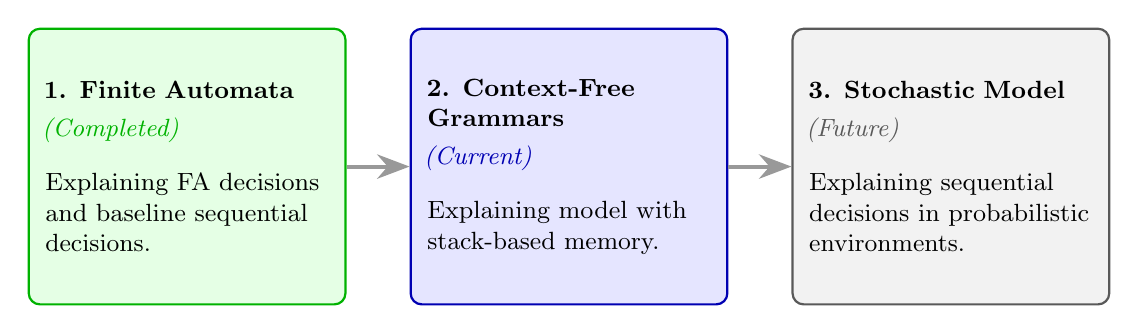
\begin{tikzpicture}[
        node distance=0.8cm,
        roadmapbox/.style={
            rectangle,
            rounded corners,
            draw,
            thick,
            text width=3.6cm, % Fits 3 boxes across a standard Beamer slide
            align=left,
            minimum height=3.5cm,
            inner sep=6pt,
            font=\small
        },
        completed/.style={roadmapbox, fill=green!10, draw=green!70!black},
        current/.style={roadmapbox, fill=blue!10, draw=blue!70!black},
        future/.style={roadmapbox, fill=gray!10, draw=gray!70!black},
        arrow/.style={-{Stealth[scale=1.2]}, line width=1.5pt, draw=gray!80}
    ]

    % --- Nodes ---
    \node[completed] (fa) {
        \textbf{1. Finite Automata}\\
        \vspace{0.1cm}
        \textit{\textcolor{green!70!black}{(Completed)}}\\[0.3cm]
        Explaining FA decisions and baseline sequential decisions.
    };

    \node[current, right=of fa] (cfg) {
        \textbf{2. Context-Free Grammars}\\
        \vspace{0.1cm}
        \textit{\textcolor{blue!70!black}{(Current)}}\\[0.3cm]
        % Explaining Context-Free Languages requiring stack-based memory.
        Explaining model with stack-based memory.
    };

    \node[future, right=of cfg] (stoch) {
        \textbf{3. Stochastic Model}\\
        \vspace{0.1cm}
        \textit{\textcolor{gray!70!black}{(Future)}}\\[0.3cm]
        Explaining sequential decisions in probabilistic environments.
    };

    % % --- Arrows ---
    \draw[arrow] (fa) -- (cfg);
    \draw[arrow] (cfg) -- (stoch);

    \end{tikzpicture}
\end{frame}

\section{Completed Work: Finite Automata}

\begin{frame}{Explaining Finite Automata (Completed)}
    \begin{itemize}
        \item FA is a mapping from an input $w \in \Sigma^*$
        to a class $\mathcal{K} = \{\text{Accept}, \text{Reject}\}$.
    \end{itemize}

    \begin{center}
    \scalebox{0.8}{
    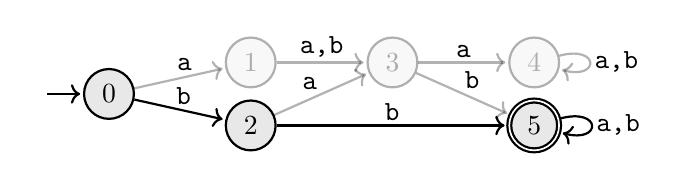
\begin{tikzpicture}[shorten >=1pt, node distance=1cm, on grid, auto, initial text=, thick]
      \tikzstyle{every state}=[fill={rgb:black,1;white,10}, minimum size=18pt, inner sep=1pt]

      % Nodes
      \node[state, initial]            (q0) {0};
      \node[state, opacity=0.3]        (q1) [right=1.8cm of q0, yshift=0.4cm] {1};
      \node[state]                     (q2) [right=1.8cm of q0, yshift=-0.4cm] {2};
      \node[state, opacity=0.3]        (q3) [right=1.8cm of q1] {3};
      \node[state, opacity=0.3]        (q4) [right=1.8cm of q3] {4};
      \node[state, accepting, double]  (q5) [right=3.6cm of q2] {5};

      % Edges
      \path[->]
        (q0) edge[draw opacity=0.3] node[xshift=8pt, yshift=-1pt] {\texttt{a}} (q1)
             edge node[xshift=-5pt, yshift=-2pt] {\texttt{b}} (q2)
        (q1) edge[draw opacity=0.3] node[yshift=-2pt] {\texttt{a,b}} (q3)
        (q2) edge node[yshift=-2pt] {\texttt{b}} (q5)
             edge[draw opacity=0.3] node[xshift=2pt, yshift=-2pt] {\texttt{a}} (q3)
        (q3) edge[draw opacity=0.3] node[yshift=-2pt] {\texttt{a}} (q4)
             edge[draw opacity=0.3] node[xshift=-3pt, yshift=-2pt] {\texttt{b}} (q5)
        (q4) edge[loop right, draw opacity=0.3] node[xshift=-2pt] {\texttt{a,b}} (q4)
        (q5) edge[loop right] node[xshift=-2pt] {\texttt{a,b}} (q5);
    \end{tikzpicture}
    }
    \end{center}

    \vspace{-0.2cm}
    % Explanations Block
    \begin{center}
    \scalebox{0.8}{ 
    \begin{tikzpicture}[
        node distance=0.2cm,
        token/.style={rectangle, draw, minimum size=0.55cm, font=\ttfamily},
        wildcard/.style={rectangle, draw, minimum size=0.55cm, font=\ttfamily},
        % FIX 1: Lock the left label widths so 'AXp' and 'CXp' take the exact same space
        label/.style={font=\small\bfseries, text width=1.5cm, align=left}, 
        % FIX 2: Lock the right text widths so the bounding box never grows or shrinks
        result/.style={font=\small, text width=6.5cm, align=left} 
    ]
        %Input word
        \node[label] (lbl_w) at (-2, 0) {Input $w$:};
        \node[token] (w1) at (0,0) {b};
        \node[token, right=of w1] (w2) {b};
        \node[token, right=of w2] (w3) {b};
        \node[token, right=of w3] (w4) {b};
        \node[token, right=of w4] (w5) {b};
        \node[result, right=0.3cm of w5] {\color{green!60!black}$\rightarrow$ Accept};


        \only<1>{
            % Abductive Explanation 1
            \node[label] (lbl_axp1) at (-2, -0.9) {AXp 1:};
            \node[token, fill=blue!10] (a1_1) at (0,-0.9) {b};
            \node[token, fill=blue!10, right=of a1_1] (a2_1) {b};
            \node[wildcard, right=of a2_1] (a3_1) {$\Sigma$};
            \node[wildcard, right=of a3_1] (a4_1) {$\Sigma$};
            \node[wildcard, right=of a4_1] (a5_1) {$\Sigma$};
            \node[result, right=0.3cm of a5_1] {\color{blue!70!black}$\rightarrow$ Guarantees Accept $L(\texttt{bb} \Sigma \Sigma \Sigma) \subseteq L(\mathcal{A})$};

            % Abductive Explanation 2
            \node[label] (lbl_axp2) at (-2, -1.8) {AXp 2:};
            \node[wildcard] (a1_2) at (0,-1.8) {$\Sigma$};
            \node[wildcard, right=of a1_2] (a2_2) {$\Sigma$};
            \node[token, fill=blue!10, right=of a2_2] (a3_2) {b};
            \node[wildcard, right=of a3_2] (a4_2) {$\Sigma$};
            \node[wildcard, right=of a4_2] (a5_2) {$\Sigma$};
            \node[result, right=0.3cm of a5_2] {\color{blue!70!black}$\rightarrow$ Guarantees Accept $L(\Sigma \Sigma \texttt{b} \Sigma \Sigma) \subseteq L(\mathcal{A})$};
        }

        \only<2>{
            % Contrastive Explanation 1 
            \node[label] (lbl_cxp1) at (-2, -0.9) {CXp 1:};
            \node[wildcard, fill=red!10] (c1_1) at (0,-0.9) {$\Sigma$};
            \node[token, right=of c1_1] (c2_1) {b};
            \node[wildcard, fill=red!10, right=of c2_1] (c3_1) {$\Sigma$};
            \node[token, right=of c3_1] (c4_1) {b};
            \node[token, right=of c4_1] (c5_1) {b};
            \node[result, right=0.3cm of c5_1] {\color{red!70!black}$\rightarrow$ Enables Reject $L(\Sigma \texttt{b} \Sigma \texttt{bb}) \not\subseteq L(\mathcal{A})$};

            % Contrastive Explanation 2
            \node[label] (lbl_cxp2) at (-2, -1.8) {CXp 2:};
            \node[token] (c1_2) at (0,-1.8) {b};
            \node[wildcard, fill=red!10, right=of c1_2] (c2_2) {$\Sigma$};
            \node[wildcard, fill=red!10, right=of c2_2] (c3_2) {$\Sigma$};
            \node[token, right=of c3_2] (c4_2) {b};
            \node[token, right=of c4_2] (c5_2) {b};
            \node[result, right=0.3cm of c5_2] {\color{red!70!black}$\rightarrow$ Enables Reject $L(\texttt{b} \Sigma \Sigma \texttt{bb}) \not\subseteq L(\mathcal{A})$};
        }
    \end{tikzpicture}
    }
    \end{center}
\end{frame}
\begin{frame}[fragile]{Why Finite Automata Are Not Enough}

    \begin{itemize}
        \item $L=\{a^{n}b^{n} \mid n \geq 1\}$ cannot be described by a FA.
        \item For a rejected word like \texttt{aaaabb},
        standard parsers identify the error at the end.
        %\item Standard parsers fail at the end of the input, obscuring the actual root cause (the extra bracket):
    \end{itemize}
    
    \vspace{0.4cm}

    \begin{columns}[T] % The [T] aligns the columns at the top
        
        % Left Column: C Code
        \begin{column}{0.48\textwidth}
            \textbf{Source Code:}
\begin{lstlisting}[language=C, basicstyle=\ttfamily\scriptsize, frame=single]
int main(){
    for(int i=0; i<10; i++){{  // Error
        printf("hello");
    }
}
\end{lstlisting}
        \end{column}

        % Right Column: Compiler Error
        \begin{column}{0.48\textwidth}
            \textbf{Parser Output:}
            % Note: Keep the verbatim text flush left so it doesn't add weird spaces
\begin{small}
\begin{verbatim}
error: expected '}' at end of input
5 | }
  |  ^
\end{verbatim}
\end{small}
        \end{column}

    \end{columns}

\end{frame}


\begin{frame}{Explaining Context-Free Grammars}
    \begin{itemize}
        \item Transition to Context-Free Grammars (CFGs).
        \item Consider $G=(\{B\}, \{\texttt{(},\texttt{)}\}, R, B)$ for balanced parentheses, with rules $R$:
    \end{itemize}
    %
    \begin{equation}
    \begin{aligned}
        B &\to \texttt{(} \, B \, \texttt{)} \, B & \text{(Rule 1)}\\
        B &\to \texttt{(} \, B \, \texttt{)} & \text{(Rule 2)}\\
        B &\to \texttt{(} \, \texttt{)} \, B & \text{(Rule 3)}\\
        B &\to \texttt{(} \, \texttt{)} & \text{(Rule 4)}
    \end{aligned}
    \end{equation}
\end{frame}


\begin{frame}{The Minimal Hitting Set Duality}
    \begin{itemize}
        \item \textbf{The Core Relationship:} Abductive and contrastive explanations share a duality \cite{axpcxp}.
        \item Every AXp is a minimal hitting set of the complete set of CXps, and vice versa.
        \item To flip a prediction (CXp), you must free at least one token from every reason that guarantees the current prediction (AXp).
    \end{itemize}

    \vspace{0.4cm}

    % TikZ Diagram: Hitting Set Duality
    \begin{center}
    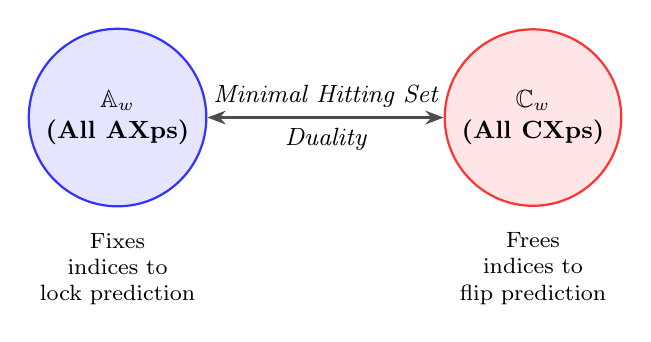
\begin{tikzpicture}[
        node distance=3cm,
        setnode/.style={circle, draw, thick, minimum size=1.5cm, align=center, font=\small\bfseries},
        arrow/.style={<->, >=Stealth, thick, draw=black!70}
    ]
        \node[setnode, fill=blue!10, draw=blue!80] (axp) {$\mathbb{A}_w$\\ (All AXps)};
        \node[setnode, fill=red!10, draw=red!80, right=of axp] (cxp) {$\mathbb{C}_w$\\ (All CXps)};
        
        \draw[arrow] (axp) -- node[above, font=\small\itshape] {Minimal Hitting Set} node[below, font=\small\itshape] {Duality} (cxp);
        
        % Little floating text blocks to explain what they do
        \node[below=0.2cm of axp, font=\footnotesize, text width=2cm, align=center] {Fixes indices to\\ lock prediction};
        \node[below=0.2cm of cxp, font=\footnotesize, text width=2cm, align=center] {Frees indices to\\ flip prediction};
    \end{tikzpicture}
    \end{center}
\end{frame} 

\begin{frame}{Outcomes: Enumeration \& Milestone}
    \begin{itemize}
        \item \textbf{Algorithmic Contribution:} 
        \begin{itemize}
            \item Leveraged this duality to develop algorithms for the formal \textbf{enumeration} of explanations in Finite Automata.
            \item Successfully maps the abstract concepts of XAI onto formal language.
        \end{itemize}
        
        \vspace{0.6cm}
        
        \begin{block}{Phase 1 Milestone Achieved}
            \textbf{Status:} Completed.\\
            \textbf{Output:} The formal definitions, duality proofs, and enumeration algorithms have been compiled and submitted to \textbf{ICALP 2026}.
        \end{block}
        
        \vspace{0.4cm}
        %\item \textit{Transitioning to Phase 2:} With the baseline for regular languages established, we now scale the complexity to languages requiring memory.
    \end{itemize}
\end{frame}


% \begin{frame}{Project Refinements Since Confirmation}
%     \textbf{Refining the Scope and Methodology:}
%     \vspace{0.3cm}
    
%     \begin{itemize}
%         \item \textbf{Shift from Automata Execution to Grammar Membership:}
%         \begin{itemize}
%             \item \textit{Initial Concept:} Explaining the execution trace and stack states of Pushdown Automata (PDA).
%             \item \textit{Refinement:} Framed the problem purely around \textbf{CFG membership} ($w \in L(G)$). This allows us to leverage efficient grammar-based parsing algorithms (like CYK) rather than tracking infinite PDA states.
%         \end{itemize}
        
%         \vspace{0.3cm}
        
%         \item \textbf{Targeted Probabilistic Scope:}
%         \begin{itemize}
%             \item \textit{Initial Concept:} Broad application to generic stochastic models.
%             \item \textit{Refinement:} Narrowed the final phase to focus specifically on Probabilistic Context-Free Grammars (PCFGs) and Markov Models, ensuring the mathematical foundation built in Phase 2 scales directly into Phase 3.
%         \end{itemize}
%     \end{itemize}
% \end{frame}

\begin{frame}
    Why $L=\{a^{n}b^{n} \mid n \geq 1\}$ cannot
    be described by a FA?

    \textbf{Intuition:}
    Finite Automata cannot count arbitrarily high because they have no external memory (like a stack).

    \textbf{Pumping Lemma for Regular Languages:}
    For any regular language,
    there is a ``pumping length'' $p$.
    If a string in the language is longer than $p$,
    the FA will get into a loop.

    If we assume $L=\{a^{n}b^{n} \mid n \geq 1\}$
    is regular, we could take a word $a^pb^p$.
    The FA must loop while reading the a's.
    This means we could "pump" (repeat) that loop of a's,
    generating a word like $a^{p+k}b^p$.
    
    The FA would still accept this new word because
    it uses the exact same path to reach the accepting
    state, but $a^{p+k}b^p$ breaks the $n=n$ rule.

    It leads to a contradiction, proving $L$ is not
    regular and cannot be described by an FA.
\end{frame}


\begin{frame}{Methodology: Parsing a word}
    \begin{itemize}
        \item The CYK algorithm requires the grammar to be in \textbf{Chomsky Normal Form} (CNF).
        \item Every rule is either $A \to BC$ (two variables) or $A \to a$ (one terminal).
        %\item This binary branching is what allows the bottom-up dynamic programming table to function.
    \end{itemize}

    \vspace{0.4cm}

    \begin{columns}[T]
        % Left Column: Original Grammar
        \begin{column}{0.48\textwidth}
            \textbf{Original Grammar ($G$):}
            \begin{equation*}
            \begin{aligned}
                B &\to \texttt{(} \, B \, \texttt{)} \, B \\
                B &\to \texttt{(} \, B \, \texttt{)} \\
                B &\to \texttt{(} \, \texttt{)} \, B \\
                B &\to \texttt{(} \, \texttt{)}
            \end{aligned}
            \end{equation*}
        \end{column}

        % Right Column: CNF Grammar
        \begin{column}{0.48\textwidth}
            \textbf{Converted CNF ($G'$):}
            \begin{equation*}
            \begin{aligned}
                B &\to N \, B & N &\to U \, R & L&\to \texttt{(}\\
                B &\to U \, R & U &\to L \, B & R&\to \texttt{)}\\
                B &\to P \, B & P &\to L \, R\\
                B &\to L \, R 
            \end{aligned}
            \end{equation*}
        \end{column}
    \end{columns}
    
    \vspace{0.4cm}
    \small{\textit{Note: We introduce variables $L$ and $R$ for the terminals, and helper variables ($N, U, P$) to break down rules longer than two symbols.}}
\end{frame}

\begin{frame}{The CYK Algorithm: Bottom-Up Parsing}
    \textbf{Input Word:} $w = \texttt{(())}$
    
    \vspace{0.2cm}
    
    \begin{columns}[T]
        \begin{column}{0.35\textwidth}
            \textbf{CNF Grammar:}
            \begin{equation*}
            \begin{aligned}
                B &\to N B \mid U R \mid P B \mid L R \\
                N &\to U R \quad U \to L B \quad P \to L R\\
                L &\to \texttt{(} \\
                R &\to \texttt{)}
            \end{aligned}
            \end{equation*}
        \end{column}
        
        \begin{column}{0.65\textwidth}
            \begin{center}
            \scalebox{0.85}{
            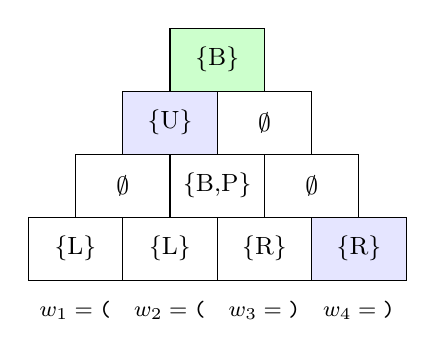
\begin{tikzpicture}[
                cell/.style={rectangle, draw, minimum width=1.2cm, minimum height=0.8cm, align=center, font=\small},
                lbl/.style={font=\footnotesize\ttfamily, text height=1.5ex, text depth=0.25ex}
            ]
                % Row 1 (Bottom - Length 1)
                \node[cell] (11) at (0,0) {\{L\}};
                \node[cell] (22) at (1.2,0) {\{L\}};
                \node[cell] (33) at (2.4,0) {\{R\}};
                \node[cell, fill=blue!10] (44) at (3.6,0) {\{R\}};
                
                % Labels below
                \node[lbl, below=0.1cm of 11] {$w_1 = \texttt{(}$};
                \node[lbl, below=0.1cm of 22] {$w_2 = \texttt{(}$};
                \node[lbl, below=0.1cm of 33] {$w_3 = \texttt{)}$};
                \node[lbl, below=0.1cm of 44] {$w_4 = \texttt{)}$};

                % Row 2 (Length 2)
                \node[cell] (12) at (0.6, 0.8) {$\emptyset$};
                \node[cell] (23) at (1.8, 0.8) {\{B,P\}};
                \node[cell] (34) at (3.0, 0.8) {$\emptyset$};

                % Row 3 (Length 3)
                \node[cell, fill=blue!10] (13) at (1.2, 1.6) {\{U\}};
                \node[cell] (24) at (2.4, 1.6) {$\emptyset$};

                % Row 4 (Top - Length 4)
                \node[cell, fill=green!20] (14) at (1.8, 2.4) {\{B\}};
                
            \end{tikzpicture}
            }
            \end{center}
        \end{column}
    \end{columns}
    
    \vspace{0.4cm}
    \small{
    \textbf{Step 1:} Initialise the base row using terminal rules ($L \to \texttt{(}$, $R \to \texttt{)}$). \\
    \textbf{Step 2:} Build upward. E.g., cell \{B\} is formed because $B \to UR$\\
    }
\end{frame}


\begin{frame}{Probabilistic Resolution of Ambiguity}
    \begin{columns}[T]
        % Bottom Left: Hypothesis A
        \begin{column}{0.5\textwidth}
            \begin{center}
                \scalebox{0.55}{
                \begin{tikzpicture}[
                    thick,
                    level distance=12mm,
                    level 1/.style={sibling distance=35mm},
                    level 2/.style={sibling distance=20mm},
                    level 3/.style={sibling distance=12mm},
                    level 4/.style={sibling distance=10mm},
                    every node/.style={font=\small}
                ]
                  \node {$B$}
                    child {node {N}
                      child {node {U}
                        child {node {$\mathbf{L}$} child {node {\texttt{(}}}}
                        child {node {$B$} 
                            child {node {$\mathbf{L}$} child {node {\texttt{(}}}} 
                            child {node {$\mathbf{R}$} child {node {\texttt{)}}}} 
                        }
                      }
                      child {node {$\mathbf{R}$} child {node {\texttt{)}}}}
                    }
                    child {node {$B$}
                      child {node {$\mathbf{L}$} child {node {\texttt{(}}}}
                      child {node {$\mathbf{R}$} child {node {\texttt{)}}}}
                    };
                \end{tikzpicture}
                }
            \end{center}
        \end{column}

        \begin{column}{0.5\textwidth}
            \begin{center}
                \scalebox{0.55}{
                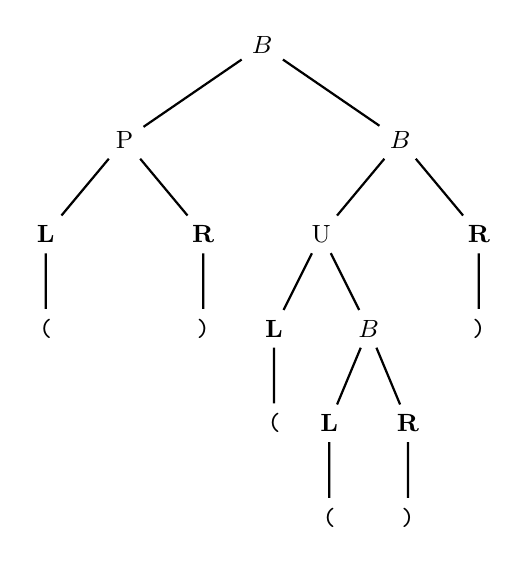
\begin{tikzpicture}[
                    thick,
                    level distance=12mm,
                    level 1/.style={sibling distance=35mm},
                    level 2/.style={sibling distance=20mm},
                    level 3/.style={sibling distance=12mm},
                    level 4/.style={sibling distance=10mm},
                    every node/.style={font=\small}
                ]
                  \node {$B$}
                    child {node {P} 
                        child {node {$\mathbf{L}$} child {node {\texttt{(}}}} 
                        child {node {$\mathbf{R}$} child {node {\texttt{)}}}} 
                    }
                    child {node {$B$}
                      child {node {U}
                        child {node {$\mathbf{L}$} child {node {\texttt{(}}}}
                        child {node {$B$} 
                            child {node {$\mathbf{L}$} child {node {\texttt{(}}}} 
                            child {node {$\mathbf{R}$} child {node {\texttt{)}}}} 
                        }
                      }
                      child {node {$\mathbf{R}$} child {node {\texttt{)}}}}
                    };
                \end{tikzpicture}
                }
            \end{center}
        \end{column}
    \end{columns}
    \begin{columns}[T]
        \begin{column}{0.5\textwidth}
            \vspace{0.1cm}
            \begin{center}
            \scalebox{0.55}{
                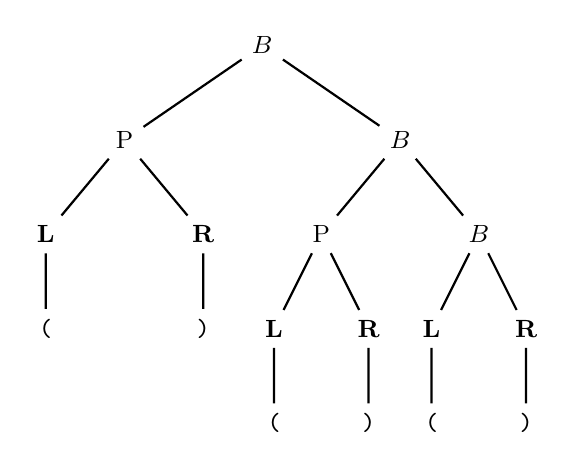
\begin{tikzpicture}[
                    thick,
                    level distance=12mm,
                    level 1/.style={sibling distance=35mm},
                    level 2/.style={sibling distance=20mm},
                    level 3/.style={sibling distance=12mm},
                    every node/.style={font=\small}
                ]
                  \node {$B$}
                    child { node {P}
                        child { node {$\mathbf{L}$} child {node {\texttt{(}}} }
                        child { node {$\mathbf{R}$} child {node {\texttt{)}}} }
                    }
                    child { node {$B$}
                        child { node {P}
                            child { node {$\mathbf{L}$} child {node {\texttt{(}}} }
                            child { node {$\mathbf{R}$} child {node {\texttt{)}}} }
                        }
                        child { node {$B$}
                            child { node {$\mathbf{L}$} child {node {\texttt{(}}} }
                            child { node {$\mathbf{R}$} child {node {\texttt{)}}} }
                        }
                    };
                \end{tikzpicture}
            }
            \end{center}
        \end{column}
        \begin{column}{0.5\textwidth}
            \vspace{0.2cm}
            \scalebox{0.75}{
                \renewcommand{\arraystretch}{1.2}
                \begin{tabular}{lcc}
                \hline
                \textbf{Rule} & \textbf{Count} & \textbf{Probability ($P$)} \\ \hline
                $B \to \mathbf{L} \ \mathbf{R}$     & 4 & $4/9 = 44.\overline{4}\%$ \\
                $B \to \text{P } B$              & 3 & $3/9 = 33.\overline{3}\%$ \\
                $B \to \text{N } B$            & 1 & $1/9 = 11.\overline{1}\%$ \\
                $B \to \text{U } \mathbf{R}$ & 1 & $1/9 = 11.\overline{1}\%$ \\ \hline
                \end{tabular}
            }
        \end{column}
    \end{columns}
\end{frame}


\begin{frame}{Explaining Finite Automata (Completed)}
    \begin{itemize}
        \item A Finite Automaton (FA) is a mapping from an input $w \in \Sigma^*$
        to a class $\mathcal{K} = \{\text{Accept}, \text{Reject}\}$.
    \end{itemize}

    \begin{center}
    \scalebox{0.8}{
    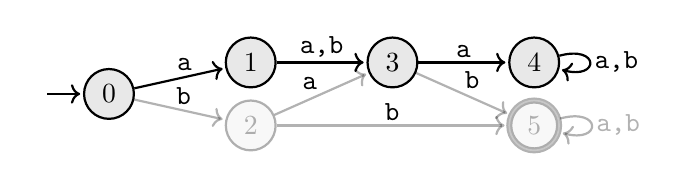
\begin{tikzpicture}[shorten >=1pt, node distance=1cm, on grid, auto, initial text=, thick]
      \tikzstyle{every state}=[fill={rgb:black,1;white,10}, minimum size=18pt, inner sep=1pt]

      % Nodes
      \node[state, initial]            (q0) {0};
      \node[state]        (q1) [right=1.8cm of q0, yshift=0.4cm] {1};
      \node[state, opacity=0.3]                     (q2) [right=1.8cm of q0, yshift=-0.4cm] {2};
      \node[state]        (q3) [right=1.8cm of q1] {3};
      \node[state]        (q4) [right=1.8cm of q3] {4};
      \node[state, accepting, double, opacity=0.3]  (q5) [right=3.6cm of q2] {5};

      % Edges
      \path[->]
        (q0) edge node[xshift=8pt, yshift=-1pt] {\texttt{a}} (q1)
             edge[draw opacity=0.3] node[xshift=-5pt, yshift=-2pt] {\texttt{b}} (q2)
        (q1) edge node[yshift=-2pt] {\texttt{a,b}} (q3)
        (q2) edge[draw opacity=0.3] node[yshift=-2pt] {\texttt{b}} (q5)
             edge[draw opacity=0.3] node[xshift=2pt, yshift=-2pt] {\texttt{a}} (q3)
        (q3) edge node[yshift=-2pt] {\texttt{a}} (q4)
             edge[draw opacity=0.3] node[xshift=-3pt, yshift=-2pt] {\texttt{b}} (q5)
        (q4) edge[loop right] node[xshift=-2pt] {\texttt{a,b}} (q4)
        (q5) edge[loop right, opacity=0.3] node[xshift=-2pt] {\texttt{a,b}} (q5);
    \end{tikzpicture}
    }
    \end{center}

    \vspace{-0.2cm}
    % Explanations Block
    \begin{center}
    \scalebox{0.8}{ 
    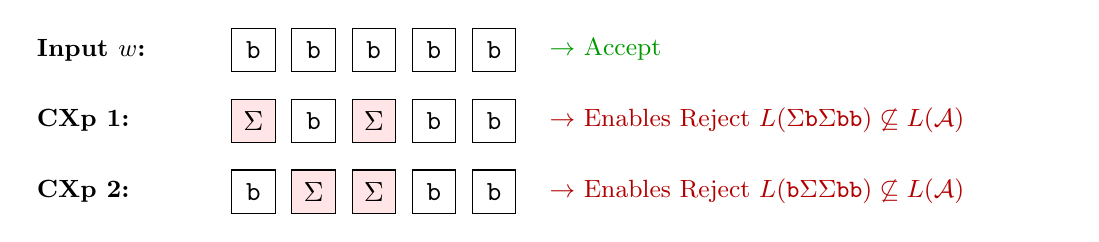
\begin{tikzpicture}[
        node distance=0.2cm,
        token/.style={rectangle, draw, minimum size=0.55cm, font=\ttfamily},
        wildcard/.style={rectangle, draw, minimum size=0.55cm, font=\ttfamily},
        % FIX 1: Lock the left label widths so 'AXp' and 'CXp' take the exact same space
        label/.style={font=\small\bfseries, text width=1.5cm, align=left}, 
        % FIX 2: Lock the right text widths so the bounding box never grows or shrinks
        result/.style={font=\small, text width=6.5cm, align=left} 
    ]
        %Input word
        \node[label] (lbl_w) at (-2, 0) {Input $w$:};
        \node[token] (w1) at (0,0) {b};
        \node[token, right=of w1] (w2) {b};
        \node[token, right=of w2] (w3) {b};
        \node[token, right=of w3] (w4) {b};
        \node[token, right=of w4] (w5) {b};
        \node[result, right=0.3cm of w5] {\color{green!60!black}$\rightarrow$ Accept};

        % Contrastive Explanation 1 
        \node[label] (lbl_cxp1) at (-2, -0.9) {CXp 1:};
        \node[wildcard, fill=red!10] (c1_1) at (0,-0.9) {$\Sigma$};
        \node[token, right=of c1_1] (c2_1) {b};
        \node[wildcard, fill=red!10, right=of c2_1] (c3_1) {$\Sigma$};
        \node[token, right=of c3_1] (c4_1) {b};
        \node[token, right=of c4_1] (c5_1) {b};
        \node[result, right=0.3cm of c5_1] {\color{red!70!black}$\rightarrow$ Enables Reject $L(\Sigma \texttt{b} \Sigma \texttt{bb}) \not\subseteq L(\mathcal{A})$};

        % Contrastive Explanation 2
        \node[label] (lbl_cxp2) at (-2, -1.8) {CXp 2:};
        \node[token] (c1_2) at (0,-1.8) {b};
        \node[wildcard, fill=red!10, right=of c1_2] (c2_2) {$\Sigma$};
        \node[wildcard, fill=red!10, right=of c2_2] (c3_2) {$\Sigma$};
        \node[token, right=of c3_2] (c4_2) {b};
        \node[token, right=of c4_2] (c5_2) {b};
        \node[result, right=0.3cm of c5_2] {\color{red!70!black}$\rightarrow$ Enables Reject $L(\texttt{b} \Sigma \Sigma \texttt{bb}) \not\subseteq L(\mathcal{A})$};
    
    \end{tikzpicture}
    }
    \end{center}
\end{frame}
%\input{example-content.tex}
\end{document}
